%%This is a very basic article template.
%%There is just one section and two subsections.
\documentclass[UTF8]{ctexart}
\title{第四章 SerDes接收端数据链路层设计}
\author{陈登}
\date{\today}

\bibliographystyle{plain}
\usepackage{graphicx}
\usepackage{float}
\usepackage{amsmath}
\usepackage{geometry}
\usepackage{fontspec}
\usepackage{algorithm}
\usepackage{algorithmicx}
\usepackage{algpseudocode}

\geometry{a4paper,centering,scale=0.9}
\usepackage[format=hang,font=small,textfont=it]{caption}
\usepackage[toc,page,title,titletoc,header]{appendix} 
\usepackage[nottoc]{tocbibind}

\newcommand\kw{\textbf}

\begin{document}

\section{SerDes接收端数据链路层设计}

\subsection{8B/10B解码器设计}

根据JESD204B协议规定,SerDes接口为保证信内数据的直流平衡,并且为了便于时钟恢复,采用8B/10B码作为数据链路层的编码方式。
JESD204B中采用的8B/10B编解码部分主要参考IEEE802.3以太网协议中关于8B/10B的编解码部分。
但是由于应用环境的不同,JESD204B协议的8B/10B编解码方式同以太网相比略有不同。

\subsubsection{协议分析}

以太网协议提供了完整的编码表,也可以看作为解码表,这几张表格的正确性毋庸置疑,是最值得参考的资料。
表中将总共268种的编码情况全部列出,可以作为校验编码正确性的基准值。

以太网协议建议,将一个码组的$RD$\footnote{Running Disparity}分为三部分,第一是上一码组计算后得出的$RD$,第二是编码后6B部分的$RD$,第三是编码后4B部分的$RD$。
而最后得到的4B部分的$RD$将作为这一组码的$RD$用于接下来码组的计算。
$RD$运算的基本结构:$last\_code\_group\_RD \to 6B\_sub-block \to 6B\_RD \to 4B\_sub-block \to 4B\_RD(new\_last\_code\_group\_RD)$。

每个sub-block的判断可用以下伪代码表示(6B和4B略有不同):

\begin{tabbing}
\qquad\=\kw{if} $000111$ or $0011$ or $1s>0s$ \\
      \>\qquad$6B\_RD=+;RD\_4B=+;$ \\
      \>\kw{else if} $111000$ or $1100$ or $1s<0s$ \\
      \>\qquad$6B\_RD=-;RD\_4B=-;$ \\
      \>\kw{else} \\
      \>\qquad$6B\_RD=last\_code\_group\_RD;$ \\
      \>\qquad$4B\_RD=6B\_RD;$ \\
      \>\kw{endif}
\end{tabbing}

最后是以太网协议中关于$RD$错误的处理,在协议附录中给出了一些接收当中的$RD$错误。
可以发现,$RD$错误是不能精确定位的,它的检测主要是通过接收机本地的$RD$和所接收到的$RD$不符所产生的错误。
但由于一系列的中性码并不会改变$RD$,前一码接收产生的错误可能因为一系列的中性码而直到几个码字后才能检测到。

在JESD204B协议中关于8B/10B编解码的规定,阅读接口协议的数据链路层内容,可以发现,在编解码器之前还有一级控制,主要是用来针对数据成帧结构中的lane、frame、multiframe的校准、同步和错误控制,而控制的依据就是解码器中获得的控制字。

在JESD204B协议中只用到了8B/10B所用控制字的5个,这将简化控制字的解码复杂度,控制字分别如下:

\begin{description}
\item[K.29.0] 即D,表示Multiframe的开始。
\item[K.28.3] 即A,表示Lane校准,一般在多帧最后出现。
\item[K.28.4] 即Q,表示Link设置数据的开始,在他之后跟一系列设置数据,配置Link,他也是ILAS\footnote{Initial Lane Alignment Sequence}的组成部分。
\item[K.28.7] 即K,表示Group同步,可以说是链接开头最重要的部分,用来保持同步,是CGS\footnote{Code Group Synchronization}的重要控制字。
\item[K.28.7] 即F,表示Frame校准,一般表示一帧结束。
\end{description}

JESD204B协议还规定了三种重要的解码错误,这些在解码器级别的错误是属于不太严重的错误,有可能经常发生,在错误并不严重的情况下并不需要进行重同步,但是需要上报给错误处理部分,供应用层决定如何处理。

错误包括以下三种:

\begin{description}
\item[Not-in-table Error] 这种错误意味着接收到的码字在任何$RD$情况下都不存在于码表中,就是一些非法的码字。对于这些码字,协议规定接收端需要重复之前收到的最新的没有错误的帧。
\item[Disparity Error] 这种错误就是上文提到的$RD$错误,协议规定解码器要根据收到的数据和$RD$直接解码。由于在检测到$RD$错误时,可能产生错误的不是这个码字,这样的处理方式也比较合理。
\item[Unexpected Control Character] 这种错误就是指未出现在指定位置的控制字,这一错误的具体处理需要由lane/frame监测部分来决定,属于接下来层级的处理,解码器并无法判断出这一错误。
\end{description}

\subsubsection{解码思路}

通过对现有论文编解码方式的理解分析,可以发现编码的方式比较多样,但解码仍主要停留在通过逻辑的方式。
在\cite{zhaoyh2003}、\cite{hecf2005}和\cite{Widmer1983}中采用的是纯逻辑解码方式;在\cite{wenl2007}和\cite{Actel1998}这两篇文章中采用的是多路选择器的方式。

在现有文章的解码中,$RD$值仅作为差错检测,这是一种对信号资源的浪费,如果通过$RD$来进行解码,可以更好的利用现有的码表。
对于已知码组的$RD$信息,可以得出下一组码可能的编码情况,这时就可以通过取反操作来压缩解码表的大小,更快的处理解码操作。
例如,已知前一组码字的$RD$信息为$RD+$,则可以推测出接下来的$6B$数据的$RD$信息只有可能为$RD-$或者均衡两种可能。
因此只需要处理一种极性的码字就可以完成对整个编码的解码,复杂度变为原来的一半。

对于数据字而言,在获知当前$RD$状态的前提下,解码就分为两种情况。
一种是相反的极性,还有一种是均衡的极性。
对于相反的极性而言,不需要对另一种极性解码,整张解码用表就可以缩小一半,一方面节约了芯片面积额,一方面提高了解码效率。
对于均衡极性而言,由\cite{Widmer1983}中编码原理分析可知,对于均衡码的解码其实非常简便,只需要输出其低$5$或$3$位。
因此,只需要设计一个均衡码判断电路,就可以快速选择是否通过解码逻辑极性解码。

对于控制字而言,由\cite{Actel1998}中提到的控制信息检测可以发现,通过$RD$和固定位置的比特就可以区分该码字是否为控制字,并且确定是哪一类控制字($K.28.x$还是$K.23.7$、$K.27.7$、$K.29.7$、$K.30.7$)。
在分析编码可知,控制字的$3B$或$5B$部分的编码规则同数据字是相同的。那么就可以“借用”数据字的解码部分来对控制字部分解码,准确输出控制码字。
其中包括了均衡和非均衡的情况,处理逻辑同数据字,唯一不同的就是控制字状态标记是否拉高。

最后对于解码模块的考虑,一般情况下都是采用的是verilog语言的case逻辑,但是对于高效的电路来说要尽量避免对语言原生性能的依赖。
通过逻辑化简的方法对更小的码表进行化简,这样的得到表达式速度更快,并且面积较小。

具体逻辑框图如图\ref{fig:8b10b_decoder_diagram}所示。

\begin{figure}[H]
\centering
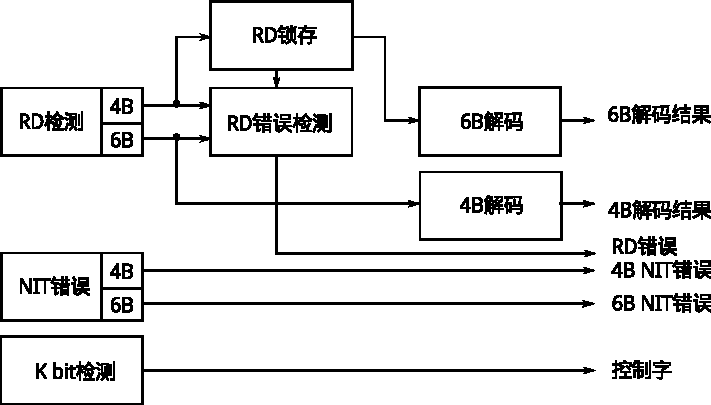
\includegraphics[width=14cm]{./img/8b10b_decoder_diagram.pdf}
\caption{SerDes接收端数据流传输结构框图}
\label{fig:8b10b_decoder_diagram}
\end{figure}

\subsubsection{第一级,预处理级}

\paragraph{K Bit检测}

根据输入完整的$10B$数据判断是否为控制信号。
有以下伪代码:

\begin{tabbing}
\qquad\=\kw{if} $iedc==1111|0000$ \\
      \>\qquad$K.28.x=1;K.x.7=0;$ \\
      \>\kw{else if} $jhgfie==010111|101000$ \\
      \>\qquad$K.28.x=0;K.x.7=1;$ \\
      \>\kw{else} \\
      \>\qquad$K.28.x=0;K.x.7=0;$ \\
      \>\kw{endif}
\end{tabbing}

本设计中的8B/10B编码,只采用了6B部分为K.28的控制字。
由完整检测逻辑可以得出,只需要检测6B部分的cdei位是否为0000或者1111,就能判断出结果。
所以判断控制字本设计可以采用最简单的逻辑表达式:

$$K\_bit = (c \& d \& e \& i)\quad|\quad~(c | d | e | i)$$

\paragraph{$6B$和$4B$平衡检测}

就是对给出的并行数据,分别输出$6B$和$4B$是否平衡,平衡即指0和1的数量是否相同。
有以下伪代码\footnote{其中$RL$表示游程长度计算,即$1$的个数。下同。}:

\begin{tabbing}
\qquad\=\kw{if} $RL(6B)==3$ \\
      \>\qquad$Balance\_6B=1;$ \\
      \>\kw{else} \\
      \>\qquad$Balance\_6B=0;$ \\
      \>\kw{endif}
\end{tabbing}

\begin{tabbing}
\qquad\=\kw{if} $RL(4B)==2$ \\
      \>\qquad$Balance\_4B=1;$ \\
      \>\kw{else} \\
      \>\qquad$Balance\_4B=0;$ \\
      \>\kw{endif}
\end{tabbing}

\paragraph{RD信息检测}

RD信息检测主要指分别计算6B和4B部分的$RD$,每一部分又分别有两个输出,$RD-$和$RD+$。
因为每一组码字的$RD$一共存在三种可能,即正、负和平衡,不属于负和正的码字,既为平衡,平衡的判断也可由上文中的伪代码确定。
这些重要的信息主要用于极性错误检测和解码。
通过对合法码字的真值表进行化简,可以得到快速RD极性检测模块,准确输出正确码字RD的负和正信号。

最终模块输出4个信号,即RD\_6B\_pos、RD\_6B\_neg、RD\_4B\_pos、RD\_4B\_neg。

\paragraph{NIT错误检测}

Not-In-Table Error的检测也分为4B和6B两部分。

6B部分的错误码字一共为14种,如表\ref{tab:tab_6B_NIT_err},参考\cite{Widmer1983}一文的方法可以分为两类,既考虑abcd全为0或全为1的情况和abcd有且仅有1个1或仅有1个0的情况。
前者直接可以判断该码字为错误码字,后者再观察ef是否全为0或全为1,也可判断码字是否错误。

4B部分的错误码字相对较为复杂,考虑到K.28中只有5个控制字是合法的,所以要对余下的码字报错。
4B部分报错情况如表\ref{tab:tab_4B_NIT_err}所示。

\begin{table}[H]
\begin{minipage}[t]{.5\textwidth}
\centering
\caption{6B码字错误情况}
\label{tab:tab_6B_NIT_err}
\begin{tabular}{|c|r|r|r|}
\hline
	abcdei	&	abcdei	\\
\hline
	000000	&	111111	\\
	000001	&	111110	\\
	000010	&	111101	\\
	000100	&	111011	\\
	001000	&	110111	\\
	010000	&	101111	\\
	100000	&	011111	\\
\hline
\end{tabular}
\end{minipage}
\begin{minipage}[t]{.5\textwidth}
\centering
\caption{4B码字错误情况}
\label{tab:tab_4B_NIT_err}
\begin{tabular}{|c|r|r|r|}
\hline
	abcdei	&	hgfj	\\
\hline
	xxxxxx	&	0000	\\
			&	1111	\\
\hline
	001111	&	0101	\\
			&	1001	\\
			&	0110	\\
\hline
	110000	&	1010	\\
			&	1001	\\
			&	0110	\\
\hline
\end{tabular}
\end{minipage}
\end{table}

\subsubsection{RD错误检测}

RD错误检测部分主要负责检测关于RD的错误,主要就是指不能出现连续相同的RD变化。
这就与寄存器中上一串码字的RD有关,所以RD错误检测还负责解码器RD的刷新。
检测可以通过RD信息计算模块提供的信号进行判断,并得到新的RD存入寄存器,如表\ref{tab:tab_RD_err}所示。

\begin{table}[H]
\centering
\caption{RD错误检测及新RD生成表}
\label{tab:tab_RD_err}
\begin{tabular}{|c|c|c|c|c|c|c|}
\hline
	last	&	6B+	&	6B-	&	4B+	&	4B-	&	err	&	new	\\
\hline
	0 	 	&	0 	&	0 	& 	0	&	0 	&	0 	&	0 	\\
	0 	 	&	0 	&	0 	& 	0	&	1 	&	1 	&	0 	\\
	0 	 	&	0 	&	0 	& 	1	&	0 	&	0 	&	1 	\\
	0 	 	&	0 	&	1 	& 	0	&	0 	&	1 	&	0 	\\
	0 	 	&	0 	&	1 	& 	0	&	1 	&	1 	&	0 	\\
	0 	 	&	0 	&	1 	& 	1	&	0 	&	1 	&	1 	\\
	0 	 	&	1 	&	0 	& 	0	&	0 	&	0 	&	1 	\\
	0 	 	&	1 	&	0 	& 	0	&	1 	&	0 	&	0 	\\
	0 	 	&	1 	&	0 	& 	1	&	0 	&	1 	&	1 	\\
	1 	 	&	0 	&	0 	& 	0	&	0 	&	0 	&	1 	\\
	1 	 	&	0 	&	0 	& 	0	&	1 	&	0 	&	0 	\\
	1 	 	&	0 	&	0 	& 	1	&	0 	&	1 	&	1 	\\
	1 	 	&	0 	&	1 	& 	0	&	0 	&	0 	&	0 	\\
	1 	 	&	0 	&	1 	& 	0	&	1 	&	1 	&	0 	\\
	1 	 	&	0 	&	1 	& 	1	&	0 	&	0 	&	1 	\\
	1 	 	&	1 	&	0 	& 	0	&	0 	&	1 	&	1 	\\
	1 	 	&	1 	&	0 	& 	0	&	1 	&	1 	&	0 	\\
	1 	 	&	1 	&	0 	& 	1	&	0 	&	1 	&	1 	\\
\hline
\end{tabular}
\end{table}

根据此表化简逻辑表达式即可得到准确的RD错误和本码字的RD情况。
为了保证时序的正确和避免未知情况的发生,参考了\cite{AlKafi2013}中的有限状态机方法来对RD进行判断、存储。

\subsubsection{第二级,解码级}

\paragraph{解码表输入级}

根据$RD$情况,对输入码字进行反转。伪代码如下:

\begin{tabbing}
\qquad\=\kw{if} $RD==RD+$ \\
      \>\qquad$6B=6B;$ \\
      \>\kw{else} \\
      \>\qquad$6B=!6B;$ \\
      \>\kw{endif}
\end{tabbing}

\begin{tabbing}
\qquad\=$RD\_6=RD|Balance\_6B$ \\
      \>\kw{if} $RD\_6==RD+$ \\
      \>\qquad$4B=4B;$ \\
      \>\kw{else} \\
      \>\qquad$4B=!4B;$ \\
      \>\kw{endif}
\end{tabbing}

\paragraph{$6B/5B$和$4B/3B$解码级}

根据解码表对输入码字解码。解码表中存的查找项均为$RD$为正时的解码,根据输入输出解码结果。

\paragraph{直接输出或解码输出选择级}

根据码字平衡与否选择是直接输出低五位还是输出查表解码后的结果。

\paragraph{控制字输出或数据字输出选择级}

根据$K.x.7$和$K.28.x$两位,选择输出控制字还是数据字。伪代码如下:

\begin{tabbing}
\qquad\=\kw{if} $K.x.7==1$ \\
      \>\qquad$8B=5B+111;K=1;$ \\
      \>\kw{else if} $K.28.x==1$ \\
      \>\qquad$8B=00111+3B;K=1;$ \\
      \>\kw{else} \\
      \>\qquad$8B=5B+3B;K=0;$ \\
      \>\kw{endif}
\end{tabbing}

不同于\cite{Actel1998}文中所描述的CASE方法,也不同于\cite{Widmer1983}中的纯逻辑方法。
本设计引入了各个模块的$RD+$信息,在读入数据之前先根据RD\_pos信息对码字进行反转。
这样,在解码时只要考虑$RD$为$RD-$和平衡的情况。
对于6B解码表由原来的48种情况减少为34种(如表\ref{tab:tab_6B_tab}所示);对于4B解码表,由于其解码需要考虑K Bit的情况,由原来的28种情况减少为16种(如表\ref{tab:tab_4B_tab}所示)。
并且由于快速的RD信息计算,使得解码模块能够更快的进行解码,缩短了解码所需时间。
最后通过逻辑化简的方法对更小的码表进行化简,这样的得到表达式速度更快,并且面积较小。

\begin{table}[H]
\begin{minipage}[t]{.5\textwidth}
\centering
\caption{6B解码表}
\label{tab:tab_6B_tab}
\begin{tabular}{|c|c|c|c|}
\hline
	abcdei	&	EDCBA	&	abcdei	&	EDCBA	\\
\hline
	000011	&	11100	&	011001	&	11001	\\
	000101	&	01111	&	011010	&	11010	\\
	000110	&	00000	&	011100	&	11100	\\
	000111	&	00111	&	100001	&	11110 	\\
	001001	&	10000	&	100010	&	11101 	\\
	001010	&	11111	&	100011	&	00011 	\\
	001011	&	01011	&	100100	&	11011 	\\
	001100	&	11000	&	100101	&	00101 	\\
	001101	&	01101	&	100110	&	00110 	\\
	001110	&	01110	&	101000	&	10111 	\\
	010001	&	00001	&	101001	&	01001 	\\
	010010	&	00010	&	101010	&	01010 	\\
	010011	&	10011	&	101100	&	01100 	\\
	010100	&	00100	&	110001	&	10001 	\\
	010101	&	10101	&	110010	&	10010 	\\
	010110	&	10110	&	110100	&	10100 	\\
	011000	&	01000	&	111000	&	00111 	\\
\hline
\end{tabular}
\end{minipage}
\begin{minipage}[t]{.5\textwidth}
\centering
\caption{4B解码表}
\label{tab:tab_4B_tab}
\begin{tabular}{|c|c|c|}
\hline
	K	&	hgfj	&	HGF	\\
\hline
	0	&	0001	&	111	\\
	0	&	0010	&	000	\\
	0	&	0011	&	011	\\
	0	&	0100	&	100	\\
	0	&	0101	&	101	\\
	0	&	0110	&	110	\\
	0	&	1000	&	111	\\
	0	&	1001	&	001	\\
	0	&	1010	&	010	\\
	0	&	1100	&	011	\\
	1	&	0001	&	111	\\
	1	&	0010	&	000	\\
	1	&	0011	&	011	\\
	1	&	0100	&	100	\\
	1	&	1010	&	101	\\
	1	&	1100	&	011	\\
\hline
\end{tabular}
\end{minipage}
\end{table}

\subsection{解扰器设计}

\subsection{Frame/Lane对齐字符检测设计}

\bibliography{../../bib/serdes}
\end{document}

